\documentclass[twoside]{book}

% Packages required by doxygen
\usepackage{fixltx2e}
\usepackage{calc}
\usepackage{doxygen}
\usepackage[export]{adjustbox} % also loads graphicx
\usepackage{graphicx}
\usepackage[utf8]{inputenc}
\usepackage{makeidx}
\usepackage{multicol}
\usepackage{multirow}
\PassOptionsToPackage{warn}{textcomp}
\usepackage{textcomp}
\usepackage[nointegrals]{wasysym}
\usepackage[table]{xcolor}

% Font selection
\usepackage[T1]{fontenc}
\usepackage[scaled=.90]{helvet}
\usepackage{courier}
\usepackage{amssymb}
\usepackage{sectsty}
\renewcommand{\familydefault}{\sfdefault}
\allsectionsfont{%
  \fontseries{bc}\selectfont%
  \color{darkgray}%
}
\renewcommand{\DoxyLabelFont}{%
  \fontseries{bc}\selectfont%
  \color{darkgray}%
}
\newcommand{\+}{\discretionary{\mbox{\scriptsize$\hookleftarrow$}}{}{}}

% Page & text layout
\usepackage{geometry}
\geometry{%
  a4paper,%
  top=2.5cm,%
  bottom=2.5cm,%
  left=2.5cm,%
  right=2.5cm%
}
\tolerance=750
\hfuzz=15pt
\hbadness=750
\setlength{\emergencystretch}{15pt}
\setlength{\parindent}{0cm}
\setlength{\parskip}{0.2cm}
\makeatletter
\renewcommand{\paragraph}{%
  \@startsection{paragraph}{4}{0ex}{-1.0ex}{1.0ex}{%
    \normalfont\normalsize\bfseries\SS@parafont%
  }%
}
\renewcommand{\subparagraph}{%
  \@startsection{subparagraph}{5}{0ex}{-1.0ex}{1.0ex}{%
    \normalfont\normalsize\bfseries\SS@subparafont%
  }%
}
\makeatother

% Headers & footers
\usepackage{fancyhdr}
\pagestyle{fancyplain}
\fancyhead[LE]{\fancyplain{}{\bfseries\thepage}}
\fancyhead[CE]{\fancyplain{}{}}
\fancyhead[RE]{\fancyplain{}{\bfseries\leftmark}}
\fancyhead[LO]{\fancyplain{}{\bfseries\rightmark}}
\fancyhead[CO]{\fancyplain{}{}}
\fancyhead[RO]{\fancyplain{}{\bfseries\thepage}}
\fancyfoot[LE]{\fancyplain{}{}}
\fancyfoot[CE]{\fancyplain{}{}}
\fancyfoot[RE]{\fancyplain{}{\bfseries\scriptsize Generated on Sun Jul 26 2015 19\+:44\+:58 for Змейка by Doxygen }}
\fancyfoot[LO]{\fancyplain{}{\bfseries\scriptsize Generated on Sun Jul 26 2015 19\+:44\+:58 for Змейка by Doxygen }}
\fancyfoot[CO]{\fancyplain{}{}}
\fancyfoot[RO]{\fancyplain{}{}}
\renewcommand{\footrulewidth}{0.4pt}
\renewcommand{\chaptermark}[1]{%
  \markboth{#1}{}%
}
\renewcommand{\sectionmark}[1]{%
  \markright{\thesection\ #1}%
}

% Indices & bibliography
\usepackage{natbib}
\usepackage[titles]{tocloft}
\setcounter{tocdepth}{3}
\setcounter{secnumdepth}{5}
\makeindex

% Hyperlinks (required, but should be loaded last)
\usepackage{ifpdf}
\ifpdf
  \usepackage[pdftex,pagebackref=true]{hyperref}
\else
  \usepackage[ps2pdf,pagebackref=true]{hyperref}
\fi
\hypersetup{%
  colorlinks=true,%
  linkcolor=blue,%
  citecolor=blue,%
  unicode%
}

% Custom commands
\newcommand{\clearemptydoublepage}{%
  \newpage{\pagestyle{empty}\cleardoublepage}%
}


%===== C O N T E N T S =====

\begin{document}

% Titlepage & ToC
\hypersetup{pageanchor=false,
             bookmarks=true,
             bookmarksnumbered=true,
             pdfencoding=unicode
            }
\pagenumbering{roman}
\begin{titlepage}
\vspace*{7cm}
\begin{center}%
{\Large Змейка }\\
\vspace*{1cm}
{\large Generated by Doxygen 1.8.9.1}\\
\vspace*{0.5cm}
{\small Sun Jul 26 2015 19:44:58}\\
\end{center}
\end{titlepage}
\clearemptydoublepage
\tableofcontents
\clearemptydoublepage
\pagenumbering{arabic}
\hypersetup{pageanchor=true}

%--- Begin generated contents ---
\chapter{Hierarchical Index}
\section{Class Hierarchy}
This inheritance list is sorted roughly, but not completely, alphabetically\+:\begin{DoxyCompactList}
\item \contentsline{section}{field}{\pageref{classfield}}{}
\item \contentsline{section}{fruit}{\pageref{classfruit}}{}
\item \contentsline{section}{game}{\pageref{classgame}}{}
\item \contentsline{section}{painter}{\pageref{classpainter}}{}
\item Q\+Main\+Window\begin{DoxyCompactList}
\item \contentsline{section}{menu}{\pageref{classmenu}}{}
\end{DoxyCompactList}
\item Q\+Open\+G\+L\+Widget\begin{DoxyCompactList}
\item \contentsline{section}{scene}{\pageref{classscene}}{}
\end{DoxyCompactList}
\item Q\+Widget\begin{DoxyCompactList}
\item \contentsline{section}{game\+Field}{\pageref{classgame_field}}{}
\end{DoxyCompactList}
\item \contentsline{section}{snake}{\pageref{classsnake}}{}
\end{DoxyCompactList}

\chapter{Class Index}
\section{Class List}
Here are the classes, structs, unions and interfaces with brief descriptions\+:\begin{DoxyCompactList}
\item\contentsline{section}{\hyperlink{classfield}{field} \\*
\begin{DoxyItemize}
\item класс описывает модель поля 
\end{DoxyItemize}}{\pageref{classfield}}{}
\item\contentsline{section}{\hyperlink{classfruit}{fruit} \\*
\begin{DoxyItemize}
\item класс описывающий фрукт 
\end{DoxyItemize}}{\pageref{classfruit}}{}
\item\contentsline{section}{\hyperlink{classgame}{game} \\*
\begin{DoxyItemize}
\item класс игры (отвечает за всю внутреигровую механику) 
\end{DoxyItemize}}{\pageref{classgame}}{}
\item\contentsline{section}{\hyperlink{classgame_field}{game\+Field} \\*
\begin{DoxyItemize}
\item класс окна игры 
\end{DoxyItemize}}{\pageref{classgame_field}}{}
\item\contentsline{section}{\hyperlink{classmenu}{menu} }{\pageref{classmenu}}{}
\item\contentsline{section}{\hyperlink{classpainter}{painter} \\*
\begin{DoxyItemize}
\item класс отображения обозначений на сцене 
\end{DoxyItemize}}{\pageref{classpainter}}{}
\item\contentsline{section}{\hyperlink{classscene}{scene} \\*
\begin{DoxyItemize}
\item класс виждета игры -\/ осуществляет управление игровы процессом и его отображение 
\end{DoxyItemize}}{\pageref{classscene}}{}
\item\contentsline{section}{\hyperlink{classsnake}{snake} \\*
\begin{DoxyItemize}
\item класс змейки 
\end{DoxyItemize}}{\pageref{classsnake}}{}
\end{DoxyCompactList}

\chapter{Class Documentation}
\hypertarget{classfield}{}\section{field Class Reference}
\label{classfield}\index{field@{field}}


The field class -\/ класс описывает модель поля  




{\ttfamily \#include $<$field.\+h$>$}

\subsection*{Public Types}
\begin{DoxyCompactItemize}
\item 
\hypertarget{classfield_a4910f59c849d43bf598b42fc47c91fba}{}enum \hyperlink{classfield_a4910f59c849d43bf598b42fc47c91fba}{Type} \{ {\bfseries E\+M\+P\+T\+Y}, 
{\bfseries S\+N\+A\+K\+E\+\_\+\+B\+L\+O\+C\+K}, 
{\bfseries F\+R\+U\+I\+T}, 
{\bfseries B\+A\+R\+R\+I\+E\+R}
 \}\label{classfield_a4910f59c849d43bf598b42fc47c91fba}

\begin{DoxyCompactList}\small\item\em The Type enum -\/ тип блока (Пустое поле, часть змеи, фрукт, препядствие) \end{DoxyCompactList}\end{DoxyCompactItemize}
\subsection*{Public Member Functions}
\begin{DoxyCompactItemize}
\item 
\hyperlink{classfield_a26b09d2e9cf52d1dca855e4b2b0ecc1c}{field} (int w, int h, bool $\ast$$\ast$f)
\begin{DoxyCompactList}\small\item\em field -\/ строит поле заданного размера с заданым набором препядствий \end{DoxyCompactList}\item 
void \hyperlink{classfield_abab6fad3d032bfbf90b01061a94ace8f}{set\+Block} (\hyperlink{classfield_a4910f59c849d43bf598b42fc47c91fba}{Type} type, int x, int y)
\begin{DoxyCompactList}\small\item\em set\+Block -\/ задать значение блока \end{DoxyCompactList}\item 
\hyperlink{classfield_a4910f59c849d43bf598b42fc47c91fba}{Type} \hyperlink{classfield_aaa9d47268100ef05881a520a0a3cd03b}{block} (int x, int y) const 
\begin{DoxyCompactList}\small\item\em block -\/ получить значение блока \end{DoxyCompactList}\item 
void \hyperlink{classfield_ae47f26cdf47b171204c3227c3246e307}{draw} (\hyperlink{classpainter}{painter} \&p) const 
\begin{DoxyCompactList}\small\item\em draw -\/ отображает заданный приметив на поле \end{DoxyCompactList}\item 
void \hyperlink{classfield_a45a3a4059cd2878eb9dba6bfb7ef6b26}{new\+O} (\hyperlink{classfield_a4910f59c849d43bf598b42fc47c91fba}{Type} t)
\begin{DoxyCompactList}\small\item\em new\+O -\/ создает новый объект заданого типа в случайной позиции \end{DoxyCompactList}\item 
\hypertarget{classfield_ae97437dfcb63a1bf1a3c5184d660581e}{}void \hyperlink{classfield_ae97437dfcb63a1bf1a3c5184d660581e}{clear} ()\label{classfield_ae97437dfcb63a1bf1a3c5184d660581e}

\begin{DoxyCompactList}\small\item\em clear -\/ отчишает поле \end{DoxyCompactList}\end{DoxyCompactItemize}
\subsection*{Static Public Member Functions}
\begin{DoxyCompactItemize}
\item 
static int \hyperlink{classfield_ad7e4bc6120a1361f6a35fd971b1f3117}{get\+W} ()
\begin{DoxyCompactList}\small\item\em get\+W -\/ получить ширину последнего созданного поля \end{DoxyCompactList}\item 
static int \hyperlink{classfield_a448b10832582b5d2d3d6d8df9ce9a900}{get\+H} ()
\begin{DoxyCompactList}\small\item\em get\+H -\/ получить высоту последнего созданного поля \end{DoxyCompactList}\end{DoxyCompactItemize}
\subsection*{Public Attributes}
\begin{DoxyCompactItemize}
\item 
\hypertarget{classfield_a289fd27a869500e67777681600857c5a}{}const int \hyperlink{classfield_a289fd27a869500e67777681600857c5a}{B\+L\+O\+C\+K\+\_\+\+W\+I\+D\+T\+H} = 10\label{classfield_a289fd27a869500e67777681600857c5a}

\begin{DoxyCompactList}\small\item\em B\+L\+O\+C\+K\+\_\+\+W\+I\+D\+T\+H -\/ ширина одного блока изображения \end{DoxyCompactList}\item 
\hypertarget{classfield_a6a662370eedab7fd586e15f1f8ee49cc}{}const int \hyperlink{classfield_a6a662370eedab7fd586e15f1f8ee49cc}{B\+L\+O\+C\+K\+\_\+\+H\+E\+I\+G\+H\+T} = 10\label{classfield_a6a662370eedab7fd586e15f1f8ee49cc}

\begin{DoxyCompactList}\small\item\em B\+L\+O\+C\+K\+\_\+\+H\+E\+I\+G\+H\+T -\/ высота одного блока изображения \end{DoxyCompactList}\end{DoxyCompactItemize}


\subsection{Detailed Description}
The field class -\/ класс описывает модель поля 

\subsection{Constructor \& Destructor Documentation}
\hypertarget{classfield_a26b09d2e9cf52d1dca855e4b2b0ecc1c}{}\index{field@{field}!field@{field}}
\index{field@{field}!field@{field}}
\subsubsection[{field}]{\setlength{\rightskip}{0pt plus 5cm}field\+::field (
\begin{DoxyParamCaption}
\item[{int}]{w, }
\item[{int}]{h, }
\item[{bool $\ast$$\ast$}]{f}
\end{DoxyParamCaption}
)}\label{classfield_a26b09d2e9cf52d1dca855e4b2b0ecc1c}


field -\/ строит поле заданного размера с заданым набором препядствий 


\begin{DoxyParams}{Parameters}
{\em w} & -\/ ширина \\
\hline
{\em h} & -\/ высота \\
\hline
{\em f} & -\/ ката препядствий \\
\hline
\end{DoxyParams}


\subsection{Member Function Documentation}
\hypertarget{classfield_aaa9d47268100ef05881a520a0a3cd03b}{}\index{field@{field}!block@{block}}
\index{block@{block}!field@{field}}
\subsubsection[{block}]{\setlength{\rightskip}{0pt plus 5cm}{\bf field\+::\+Type} field\+::block (
\begin{DoxyParamCaption}
\item[{int}]{x, }
\item[{int}]{y}
\end{DoxyParamCaption}
) const}\label{classfield_aaa9d47268100ef05881a520a0a3cd03b}


block -\/ получить значение блока 


\begin{DoxyParams}{Parameters}
{\em x} & -\/ положение по горизонтали \\
\hline
{\em y} & -\/ положение по вертикали \\
\hline
\end{DoxyParams}
\begin{DoxyReturn}{Returns}
-\/ тип блока 
\end{DoxyReturn}
\hypertarget{classfield_ae47f26cdf47b171204c3227c3246e307}{}\index{field@{field}!draw@{draw}}
\index{draw@{draw}!field@{field}}
\subsubsection[{draw}]{\setlength{\rightskip}{0pt plus 5cm}void field\+::draw (
\begin{DoxyParamCaption}
\item[{{\bf painter} \&}]{p}
\end{DoxyParamCaption}
) const}\label{classfield_ae47f26cdf47b171204c3227c3246e307}


draw -\/ отображает заданный приметив на поле 


\begin{DoxyParams}{Parameters}
{\em p} & -\/ приметив \\
\hline
\end{DoxyParams}
\hypertarget{classfield_a448b10832582b5d2d3d6d8df9ce9a900}{}\index{field@{field}!get\+H@{get\+H}}
\index{get\+H@{get\+H}!field@{field}}
\subsubsection[{get\+H}]{\setlength{\rightskip}{0pt plus 5cm}int field\+::get\+H (
\begin{DoxyParamCaption}
{}
\end{DoxyParamCaption}
)\hspace{0.3cm}{\ttfamily [static]}}\label{classfield_a448b10832582b5d2d3d6d8df9ce9a900}


get\+H -\/ получить высоту последнего созданного поля 

\begin{DoxyReturn}{Returns}
высота 
\end{DoxyReturn}
\hypertarget{classfield_ad7e4bc6120a1361f6a35fd971b1f3117}{}\index{field@{field}!get\+W@{get\+W}}
\index{get\+W@{get\+W}!field@{field}}
\subsubsection[{get\+W}]{\setlength{\rightskip}{0pt plus 5cm}int field\+::get\+W (
\begin{DoxyParamCaption}
{}
\end{DoxyParamCaption}
)\hspace{0.3cm}{\ttfamily [static]}}\label{classfield_ad7e4bc6120a1361f6a35fd971b1f3117}


get\+W -\/ получить ширину последнего созданного поля 

\begin{DoxyReturn}{Returns}
ширина 
\end{DoxyReturn}
\hypertarget{classfield_a45a3a4059cd2878eb9dba6bfb7ef6b26}{}\index{field@{field}!new\+O@{new\+O}}
\index{new\+O@{new\+O}!field@{field}}
\subsubsection[{new\+O}]{\setlength{\rightskip}{0pt plus 5cm}void field\+::new\+O (
\begin{DoxyParamCaption}
\item[{{\bf field\+::\+Type}}]{t}
\end{DoxyParamCaption}
)}\label{classfield_a45a3a4059cd2878eb9dba6bfb7ef6b26}


new\+O -\/ создает новый объект заданого типа в случайной позиции 


\begin{DoxyParams}{Parameters}
{\em t} & -\/ тип \\
\hline
\end{DoxyParams}
\hypertarget{classfield_abab6fad3d032bfbf90b01061a94ace8f}{}\index{field@{field}!set\+Block@{set\+Block}}
\index{set\+Block@{set\+Block}!field@{field}}
\subsubsection[{set\+Block}]{\setlength{\rightskip}{0pt plus 5cm}void field\+::set\+Block (
\begin{DoxyParamCaption}
\item[{{\bf field\+::\+Type}}]{type, }
\item[{int}]{x, }
\item[{int}]{y}
\end{DoxyParamCaption}
)}\label{classfield_abab6fad3d032bfbf90b01061a94ace8f}


set\+Block -\/ задать значение блока 


\begin{DoxyParams}{Parameters}
{\em type} & -\/ тип блока \\
\hline
{\em x} & -\/ положение по горизонтали \\
\hline
{\em y} & -\/ положение по вертикали \\
\hline
\end{DoxyParams}


The documentation for this class was generated from the following files\+:\begin{DoxyCompactItemize}
\item 
field.\+h\item 
field.\+cpp\end{DoxyCompactItemize}

\hypertarget{classfruit}{}\section{fruit Class Reference}
\label{classfruit}\index{fruit@{fruit}}


The fruit class -\/ класс описывающий фрукт  




{\ttfamily \#include $<$fruit.\+h$>$}

\subsection*{Public Member Functions}
\begin{DoxyCompactItemize}
\item 
\hyperlink{classfruit_a9978303f68a9b5784e4ff61f9019b542}{fruit} (int x=0, int y=0)
\begin{DoxyCompactList}\small\item\em fruit -\/ создает фрукт с задаными координатами \end{DoxyCompactList}\item 
bool \hyperlink{classfruit_a6042abec9ccd88227de84baa24cc73db}{draw} (\hyperlink{classfield}{field} \&) const 
\begin{DoxyCompactList}\small\item\em draw -\/ отображает фрукт на поле \end{DoxyCompactList}\end{DoxyCompactItemize}


\subsection{Detailed Description}
The fruit class -\/ класс описывающий фрукт 

\subsection{Constructor \& Destructor Documentation}
\hypertarget{classfruit_a9978303f68a9b5784e4ff61f9019b542}{}\index{fruit@{fruit}!fruit@{fruit}}
\index{fruit@{fruit}!fruit@{fruit}}
\subsubsection[{fruit}]{\setlength{\rightskip}{0pt plus 5cm}fruit\+::fruit (
\begin{DoxyParamCaption}
\item[{int}]{x = {\ttfamily 0}, }
\item[{int}]{y = {\ttfamily 0}}
\end{DoxyParamCaption}
)}\label{classfruit_a9978303f68a9b5784e4ff61f9019b542}


fruit -\/ создает фрукт с задаными координатами 


\begin{DoxyParams}{Parameters}
{\em x} & \\
\hline
{\em y} & \\
\hline
\end{DoxyParams}


\subsection{Member Function Documentation}
\hypertarget{classfruit_a6042abec9ccd88227de84baa24cc73db}{}\index{fruit@{fruit}!draw@{draw}}
\index{draw@{draw}!fruit@{fruit}}
\subsubsection[{draw}]{\setlength{\rightskip}{0pt plus 5cm}bool fruit\+::draw (
\begin{DoxyParamCaption}
\item[{{\bf field} \&}]{f}
\end{DoxyParamCaption}
) const}\label{classfruit_a6042abec9ccd88227de84baa24cc73db}


draw -\/ отображает фрукт на поле 

\begin{DoxyReturn}{Returns}
успешность 
\end{DoxyReturn}


The documentation for this class was generated from the following files\+:\begin{DoxyCompactItemize}
\item 
fruit.\+h\item 
fruit.\+cpp\end{DoxyCompactItemize}

\hypertarget{classgame}{}\section{game Class Reference}
\label{classgame}\index{game@{game}}


The game class -\/ класс игры (отвечает за всю внутреигровую механику)  




{\ttfamily \#include $<$game.\+h$>$}

\subsection*{Public Member Functions}
\begin{DoxyCompactItemize}
\item 
\hyperlink{classgame_a5cd0e53cd7390f67ab998a79dd4845a3}{game} (int w, int h, bool $\ast$$\ast$f)
\begin{DoxyCompactList}\small\item\em game конструктор, который создает игру с полем заданого размера и заданной фактуры \end{DoxyCompactList}\item 
\hypertarget{classgame_af5c426af77aebd8a30262985461d5db9}{}void \hyperlink{classgame_af5c426af77aebd8a30262985461d5db9}{new\+Game} ()\label{classgame_af5c426af77aebd8a30262985461d5db9}

\begin{DoxyCompactList}\small\item\em new\+Game -\/ начинает новую игру на проинициализированном поле \end{DoxyCompactList}\item 
\hypertarget{classgame_a09def2438c9cd99bbb6de50cbb522b6f}{}void \hyperlink{classgame_a09def2438c9cd99bbb6de50cbb522b6f}{tick} ()\label{classgame_a09def2438c9cd99bbb6de50cbb522b6f}

\begin{DoxyCompactList}\small\item\em tick -\/ обрабатывает каждое новое срабатывание таймера \end{DoxyCompactList}\item 
void \hyperlink{classgame_a4942c71770f579508e3e2ea6bc066fbe}{draw} (\hyperlink{classpainter}{painter} \&p) const 
\begin{DoxyCompactList}\small\item\em draw -\/ рисует на поле обект класса painter(примитив) \end{DoxyCompactList}\item 
\hypertarget{classgame_ae01f3a26ab769ed793f380f0fc9cfa4b}{}void \hyperlink{classgame_ae01f3a26ab769ed793f380f0fc9cfa4b}{key\+Event} (\hyperlink{classsnake_adbd63ec22af655a4827ae26c7b9f5216}{snake\+::\+Direction})\label{classgame_ae01f3a26ab769ed793f380f0fc9cfa4b}

\begin{DoxyCompactList}\small\item\em key\+Event -\/ передает змейки управляющий сигнал \end{DoxyCompactList}\item 
\hyperlink{classsnake_a490fdfa738dec404d2fea835645d66c2}{snake\+::\+Status} \hyperlink{classgame_a67d16ee5508076509620a60dee4ea563}{status} () const 
\begin{DoxyCompactList}\small\item\em status -\/ получает статус игры \end{DoxyCompactList}\item 
size\+\_\+t \hyperlink{classgame_afee56f47b45d78977b9f618eca139e24}{snake\+Size} () const 
\begin{DoxyCompactList}\small\item\em snake\+Size -\/ получает текущий размер змеи \end{DoxyCompactList}\item 
size\+\_\+t \hyperlink{classgame_a358a5222aa8e120023a93ebec70d2ddf}{snake\+Max\+Size} () const 
\begin{DoxyCompactList}\small\item\em snake\+Max\+Size -\/ получает максимальный размер змеии \end{DoxyCompactList}\end{DoxyCompactItemize}


\subsection{Detailed Description}
The game class -\/ класс игры (отвечает за всю внутреигровую механику) 

\subsection{Constructor \& Destructor Documentation}
\hypertarget{classgame_a5cd0e53cd7390f67ab998a79dd4845a3}{}\index{game@{game}!game@{game}}
\index{game@{game}!game@{game}}
\subsubsection[{game}]{\setlength{\rightskip}{0pt plus 5cm}game\+::game (
\begin{DoxyParamCaption}
\item[{int}]{w, }
\item[{int}]{h, }
\item[{bool $\ast$$\ast$}]{f}
\end{DoxyParamCaption}
)}\label{classgame_a5cd0e53cd7390f67ab998a79dd4845a3}


game конструктор, который создает игру с полем заданого размера и заданной фактуры 


\begin{DoxyParams}{Parameters}
{\em w} & -\/ ширина \\
\hline
{\em h} & -\/ высота \\
\hline
{\em f} & -\/ карта препядствий \\
\hline
\end{DoxyParams}


\subsection{Member Function Documentation}
\hypertarget{classgame_a4942c71770f579508e3e2ea6bc066fbe}{}\index{game@{game}!draw@{draw}}
\index{draw@{draw}!game@{game}}
\subsubsection[{draw}]{\setlength{\rightskip}{0pt plus 5cm}void game\+::draw (
\begin{DoxyParamCaption}
\item[{{\bf painter} \&}]{p}
\end{DoxyParamCaption}
) const}\label{classgame_a4942c71770f579508e3e2ea6bc066fbe}


draw -\/ рисует на поле обект класса painter(примитив) 


\begin{DoxyParams}{Parameters}
{\em p} & -\/ отображаемый примитив \\
\hline
\end{DoxyParams}
\hypertarget{classgame_a358a5222aa8e120023a93ebec70d2ddf}{}\index{game@{game}!snake\+Max\+Size@{snake\+Max\+Size}}
\index{snake\+Max\+Size@{snake\+Max\+Size}!game@{game}}
\subsubsection[{snake\+Max\+Size}]{\setlength{\rightskip}{0pt plus 5cm}size\+\_\+t game\+::snake\+Max\+Size (
\begin{DoxyParamCaption}
{}
\end{DoxyParamCaption}
) const}\label{classgame_a358a5222aa8e120023a93ebec70d2ddf}


snake\+Max\+Size -\/ получает максимальный размер змеии 

\begin{DoxyReturn}{Returns}
-\/ размер 
\end{DoxyReturn}
\hypertarget{classgame_afee56f47b45d78977b9f618eca139e24}{}\index{game@{game}!snake\+Size@{snake\+Size}}
\index{snake\+Size@{snake\+Size}!game@{game}}
\subsubsection[{snake\+Size}]{\setlength{\rightskip}{0pt plus 5cm}size\+\_\+t game\+::snake\+Size (
\begin{DoxyParamCaption}
{}
\end{DoxyParamCaption}
) const}\label{classgame_afee56f47b45d78977b9f618eca139e24}


snake\+Size -\/ получает текущий размер змеи 

\begin{DoxyReturn}{Returns}
-\/ размер 
\end{DoxyReturn}
\hypertarget{classgame_a67d16ee5508076509620a60dee4ea563}{}\index{game@{game}!status@{status}}
\index{status@{status}!game@{game}}
\subsubsection[{status}]{\setlength{\rightskip}{0pt plus 5cm}{\bf snake\+::\+Status} game\+::status (
\begin{DoxyParamCaption}
{}
\end{DoxyParamCaption}
) const}\label{classgame_a67d16ee5508076509620a60dee4ea563}


status -\/ получает статус игры 

\begin{DoxyReturn}{Returns}

\end{DoxyReturn}


The documentation for this class was generated from the following files\+:\begin{DoxyCompactItemize}
\item 
game.\+h\item 
game.\+cpp\end{DoxyCompactItemize}

\hypertarget{classgame_field}{}\section{game\+Field Class Reference}
\label{classgame_field}\index{game\+Field@{game\+Field}}


The \hyperlink{classgame_field}{game\+Field} class -\/ класс окна игры  




{\ttfamily \#include $<$gamefield.\+h$>$}

Inheritance diagram for game\+Field\+:\begin{figure}[H]
\begin{center}
\leavevmode
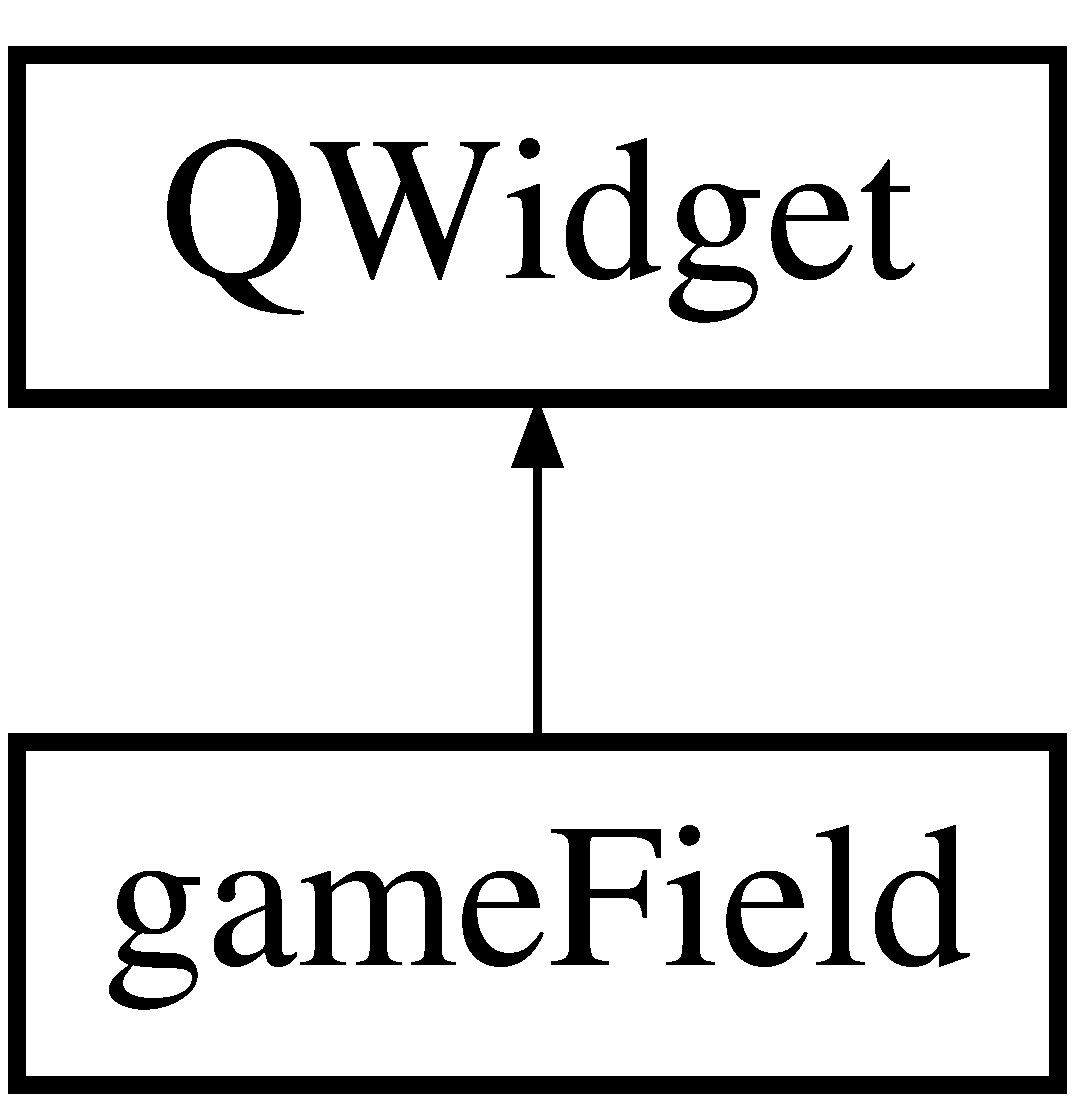
\includegraphics[height=2.000000cm]{classgame_field}
\end{center}
\end{figure}
\subsection*{Public Member Functions}
\begin{DoxyCompactItemize}
\item 
\hyperlink{classgame_field_a05df0a3ac3527b26bad66d483014190f}{game\+Field} (int w, int h, int s, bool $\ast$$\ast$f=0, Q\+Widget $\ast$parent=0)
\begin{DoxyCompactList}\small\item\em \hyperlink{classgame_field}{game\+Field} -\/ создает игры по переданным конфигурациям \end{DoxyCompactList}\end{DoxyCompactItemize}


\subsection{Detailed Description}
The \hyperlink{classgame_field}{game\+Field} class -\/ класс окна игры 

\subsection{Constructor \& Destructor Documentation}
\hypertarget{classgame_field_a05df0a3ac3527b26bad66d483014190f}{}\index{game\+Field@{game\+Field}!game\+Field@{game\+Field}}
\index{game\+Field@{game\+Field}!game\+Field@{game\+Field}}
\subsubsection[{game\+Field}]{\setlength{\rightskip}{0pt plus 5cm}game\+Field\+::game\+Field (
\begin{DoxyParamCaption}
\item[{int}]{w, }
\item[{int}]{h, }
\item[{int}]{s, }
\item[{bool $\ast$$\ast$}]{f = {\ttfamily 0}, }
\item[{Q\+Widget $\ast$}]{parent = {\ttfamily 0}}
\end{DoxyParamCaption}
)\hspace{0.3cm}{\ttfamily [explicit]}}\label{classgame_field_a05df0a3ac3527b26bad66d483014190f}


\hyperlink{classgame_field}{game\+Field} -\/ создает игры по переданным конфигурациям 


\begin{DoxyParams}{Parameters}
{\em w} & -\/ ширина поля \\
\hline
{\em h} & -\/ высота поля \\
\hline
{\em s} & -\/ скорость игры \\
\hline
{\em f} & -\/ заданные препядствия \\
\hline
{\em parent} & -\/ родительский виджет \\
\hline
\end{DoxyParams}


The documentation for this class was generated from the following files\+:\begin{DoxyCompactItemize}
\item 
gamefield.\+h\item 
gamefield.\+cpp\end{DoxyCompactItemize}

\hypertarget{classmenu}{}\section{menu Class Reference}
\label{classmenu}\index{menu@{menu}}
Inheritance diagram for menu\+:\begin{figure}[H]
\begin{center}
\leavevmode
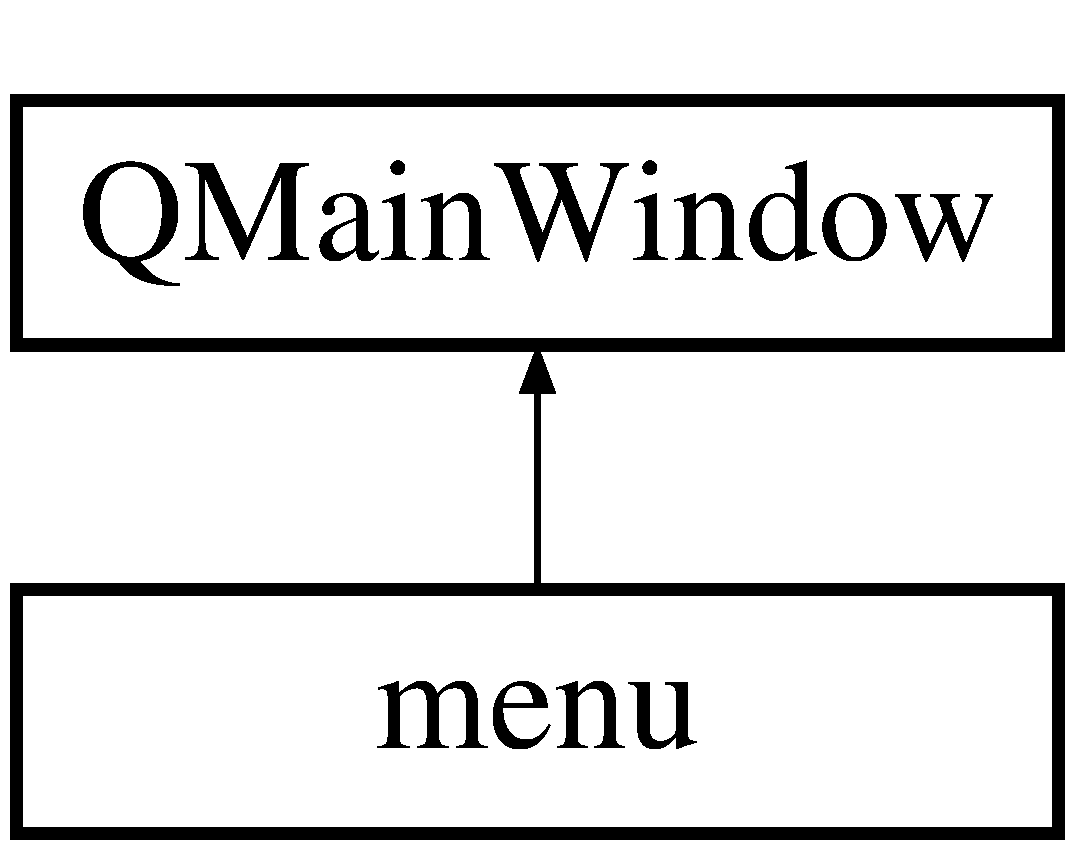
\includegraphics[height=2.000000cm]{classmenu}
\end{center}
\end{figure}
\subsection*{Public Member Functions}
\begin{DoxyCompactItemize}
\item 
\hypertarget{classmenu_aff7946ea9349eacaede63417ecea19cc}{}{\bfseries menu} (Q\+Widget $\ast$parent=0)\label{classmenu_aff7946ea9349eacaede63417ecea19cc}

\end{DoxyCompactItemize}


The documentation for this class was generated from the following files\+:\begin{DoxyCompactItemize}
\item 
menu.\+h\item 
menu.\+cpp\end{DoxyCompactItemize}

\hypertarget{classpainter}{}\section{painter Class Reference}
\label{classpainter}\index{painter@{painter}}


The painter class -\/ класс отображения обозначений на сцене  




{\ttfamily \#include $<$painter.\+h$>$}

\subsection*{Public Member Functions}
\begin{DoxyCompactItemize}
\item 
\hyperlink{classpainter_ad2449966024bf01eaca7e51dbe811ee8}{painter} (Q\+Open\+G\+L\+Shader\+Program $\ast$program)
\begin{DoxyCompactList}\small\item\em painter -\/ конструктор \end{DoxyCompactList}\item 
void \hyperlink{classpainter_a9032c525a037d38fd675b18b03cd2edb}{bar} (int x1, int y1, int x2, int y2, bool is\+Green)
\begin{DoxyCompactList}\small\item\em bar -\/ функция отрисовки квадрата заданного цвета в заданной позиции \end{DoxyCompactList}\item 
void \hyperlink{classpainter_a2f0e1b6f2820c941de240d91f0a83de7}{circle} (int x, int y, int radius)
\begin{DoxyCompactList}\small\item\em circle -\/ функция отрисовки круга(ромба) красного цвета с заданым центром и радиусом \end{DoxyCompactList}\end{DoxyCompactItemize}


\subsection{Detailed Description}
The painter class -\/ класс отображения обозначений на сцене 

\subsection{Constructor \& Destructor Documentation}
\hypertarget{classpainter_ad2449966024bf01eaca7e51dbe811ee8}{}\index{painter@{painter}!painter@{painter}}
\index{painter@{painter}!painter@{painter}}
\subsubsection[{painter}]{\setlength{\rightskip}{0pt plus 5cm}painter\+::painter (
\begin{DoxyParamCaption}
\item[{Q\+Open\+G\+L\+Shader\+Program $\ast$}]{program}
\end{DoxyParamCaption}
)}\label{classpainter_ad2449966024bf01eaca7e51dbe811ee8}


painter -\/ конструктор 


\begin{DoxyParams}{Parameters}
{\em program} & -\/ шейдерная программа \\
\hline
\end{DoxyParams}


\subsection{Member Function Documentation}
\hypertarget{classpainter_a9032c525a037d38fd675b18b03cd2edb}{}\index{painter@{painter}!bar@{bar}}
\index{bar@{bar}!painter@{painter}}
\subsubsection[{bar}]{\setlength{\rightskip}{0pt plus 5cm}void painter\+::bar (
\begin{DoxyParamCaption}
\item[{int}]{x1, }
\item[{int}]{y1, }
\item[{int}]{x2, }
\item[{int}]{y2, }
\item[{bool}]{is\+Green}
\end{DoxyParamCaption}
)}\label{classpainter_a9032c525a037d38fd675b18b03cd2edb}


bar -\/ функция отрисовки квадрата заданного цвета в заданной позиции 


\begin{DoxyParams}{Parameters}
{\em x1} & -\/ горизонтальная координата левого верхнего угла \\
\hline
{\em y1} & -\/ вертикальная координата левого верхнего угла \\
\hline
{\em x2} & -\/ горизонтальная координата правого нижнего угла \\
\hline
{\em y2} & -\/ вертикальная координата правого нижнего угла \\
\hline
{\em is\+Green} & -\/ флаг цвета (если флаг поднят то отрисовывается зеленая фигура, иначе коричьневая) \\
\hline
\end{DoxyParams}
\hypertarget{classpainter_a2f0e1b6f2820c941de240d91f0a83de7}{}\index{painter@{painter}!circle@{circle}}
\index{circle@{circle}!painter@{painter}}
\subsubsection[{circle}]{\setlength{\rightskip}{0pt plus 5cm}void painter\+::circle (
\begin{DoxyParamCaption}
\item[{int}]{x, }
\item[{int}]{y, }
\item[{int}]{radius}
\end{DoxyParamCaption}
)}\label{classpainter_a2f0e1b6f2820c941de240d91f0a83de7}


circle -\/ функция отрисовки круга(ромба) красного цвета с заданым центром и радиусом 


\begin{DoxyParams}{Parameters}
{\em x} & -\/ горизонтальная координата центра \\
\hline
{\em y} & -\/ вертикальная координата центра \\
\hline
{\em radius} & -\/ радиус \\
\hline
\end{DoxyParams}


The documentation for this class was generated from the following files\+:\begin{DoxyCompactItemize}
\item 
painter.\+h\item 
painter.\+cpp\end{DoxyCompactItemize}

\hypertarget{classscene}{}\section{scene Class Reference}
\label{classscene}\index{scene@{scene}}


The scene class -\/ класс виждета игры -\/ осуществляет управление игровы процессом и его отображение  




{\ttfamily \#include $<$scene.\+h$>$}

Inheritance diagram for scene\+:\begin{figure}[H]
\begin{center}
\leavevmode
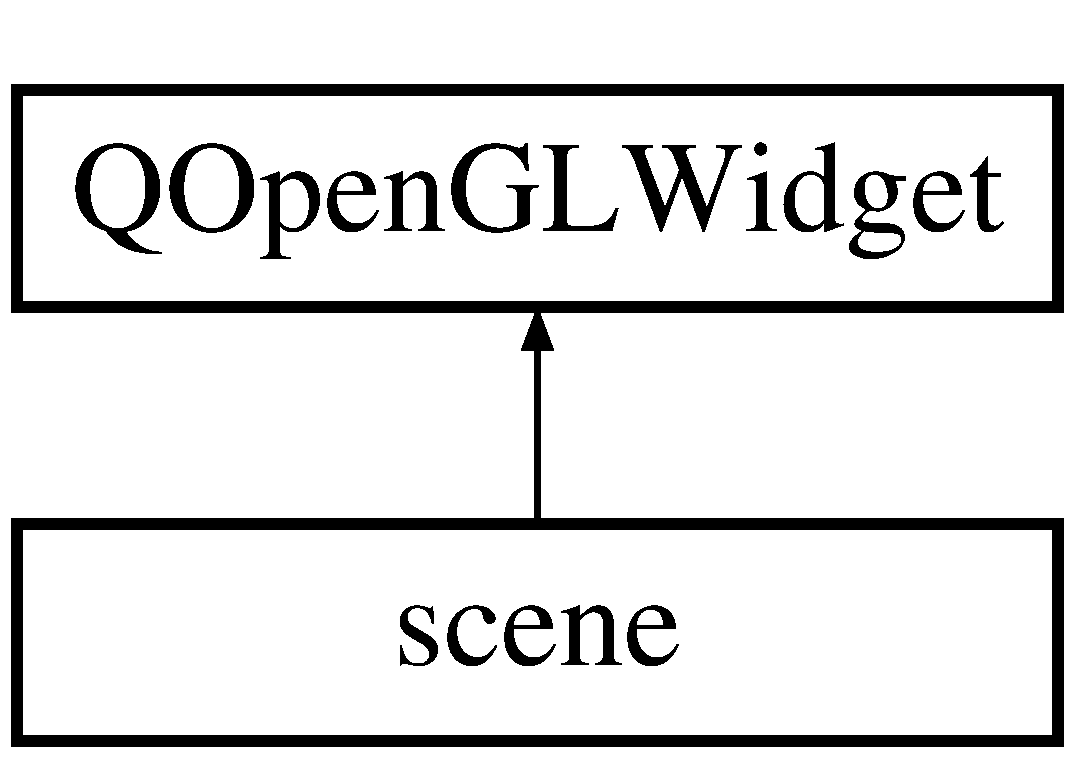
\includegraphics[height=2.000000cm]{classscene}
\end{center}
\end{figure}
\subsection*{Signals}
\begin{DoxyCompactItemize}
\item 
void \hyperlink{classscene_a63ee03bf6251756564be417b7ebd5ef5}{signal\+Show\+Status} (const Q\+String \&status)
\begin{DoxyCompactList}\small\item\em signal\+Show\+Status -\/ сигнал для передачи сообщеният в статусную строку \end{DoxyCompactList}\end{DoxyCompactItemize}
\subsection*{Public Member Functions}
\begin{DoxyCompactItemize}
\item 
\hypertarget{classscene_ac93fe52e7b2f23b16705b6cd79ab3d66}{}{\bfseries scene} (Q\+Widget $\ast$parent=0)\label{classscene_ac93fe52e7b2f23b16705b6cd79ab3d66}

\item 
void \hyperlink{classscene_a3a5609dc2e28d4541c5f2e10b5103ef3}{set\+Size} (int w\+S, int h\+S, int s, bool $\ast$$\ast$f)
\begin{DoxyCompactList}\small\item\em set\+Size -\/ передает основные игровые параметры объекту игры \end{DoxyCompactList}\end{DoxyCompactItemize}


\subsection{Detailed Description}
The scene class -\/ класс виждета игры -\/ осуществляет управление игровы процессом и его отображение 

\subsection{Member Function Documentation}
\hypertarget{classscene_a3a5609dc2e28d4541c5f2e10b5103ef3}{}\index{scene@{scene}!set\+Size@{set\+Size}}
\index{set\+Size@{set\+Size}!scene@{scene}}
\subsubsection[{set\+Size}]{\setlength{\rightskip}{0pt plus 5cm}void scene\+::set\+Size (
\begin{DoxyParamCaption}
\item[{int}]{w\+S, }
\item[{int}]{h\+S, }
\item[{int}]{s, }
\item[{bool $\ast$$\ast$}]{f}
\end{DoxyParamCaption}
)}\label{classscene_a3a5609dc2e28d4541c5f2e10b5103ef3}


set\+Size -\/ передает основные игровые параметры объекту игры 


\begin{DoxyParams}{Parameters}
{\em w\+S} & -\/ ширина поля \\
\hline
{\em h\+S} & -\/ высота поля \\
\hline
{\em s} & -\/ временной промежуток обновления таймера \\
\hline
{\em f} & -\/ карта препядствий \\
\hline
\end{DoxyParams}
\hypertarget{classscene_a63ee03bf6251756564be417b7ebd5ef5}{}\index{scene@{scene}!signal\+Show\+Status@{signal\+Show\+Status}}
\index{signal\+Show\+Status@{signal\+Show\+Status}!scene@{scene}}
\subsubsection[{signal\+Show\+Status}]{\setlength{\rightskip}{0pt plus 5cm}void scene\+::signal\+Show\+Status (
\begin{DoxyParamCaption}
\item[{const Q\+String \&}]{status}
\end{DoxyParamCaption}
)\hspace{0.3cm}{\ttfamily [signal]}}\label{classscene_a63ee03bf6251756564be417b7ebd5ef5}


signal\+Show\+Status -\/ сигнал для передачи сообщеният в статусную строку 


\begin{DoxyParams}{Parameters}
{\em status} & -\/ сообщение \\
\hline
\end{DoxyParams}


The documentation for this class was generated from the following files\+:\begin{DoxyCompactItemize}
\item 
scene.\+h\item 
scene.\+cpp\end{DoxyCompactItemize}

\hypertarget{classsnake}{}\section{snake Class Reference}
\label{classsnake}\index{snake@{snake}}


The snake class -\/ класс змейки  




{\ttfamily \#include $<$Snake.\+h$>$}

\subsection*{Public Types}
\begin{DoxyCompactItemize}
\item 
\hypertarget{classsnake_a490fdfa738dec404d2fea835645d66c2}{}enum \hyperlink{classsnake_a490fdfa738dec404d2fea835645d66c2}{Status} \{ {\bfseries I\+N\+C\+R\+E\+A\+S\+E\+D}, 
{\bfseries L\+I\+V\+E}, 
{\bfseries W\+I\+N}, 
{\bfseries D\+E\+A\+D}
 \}\label{classsnake_a490fdfa738dec404d2fea835645d66c2}

\begin{DoxyCompactList}\small\item\em The Status enum -\/ перечисление статусов змейки \end{DoxyCompactList}\item 
\hypertarget{classsnake_adbd63ec22af655a4827ae26c7b9f5216}{}enum \hyperlink{classsnake_adbd63ec22af655a4827ae26c7b9f5216}{Direction} \{ {\bfseries L\+E\+F\+T}, 
{\bfseries U\+P}, 
{\bfseries R\+I\+G\+H\+T}, 
{\bfseries D\+O\+W\+N}
 \}\label{classsnake_adbd63ec22af655a4827ae26c7b9f5216}

\begin{DoxyCompactList}\small\item\em The Direction enum -\/ типы управляющих сигналов \end{DoxyCompactList}\end{DoxyCompactItemize}
\subsection*{Public Member Functions}
\begin{DoxyCompactItemize}
\item 
\hypertarget{classsnake_aebbd5eaa3883afef2f04ac6fdeef8f16}{}\hyperlink{classsnake_aebbd5eaa3883afef2f04ac6fdeef8f16}{snake} ()\label{classsnake_aebbd5eaa3883afef2f04ac6fdeef8f16}

\begin{DoxyCompactList}\small\item\em snake -\/ конструктор по умолчанию \end{DoxyCompactList}\item 
void \hyperlink{classsnake_a30f284fce27e7a341f5b2ca4c7f92205}{tick} (\hyperlink{classfield}{field} \&f)
\begin{DoxyCompactList}\small\item\em tick -\/ обработчик таймера \end{DoxyCompactList}\item 
\hypertarget{classsnake_a3a64ec5039d750a8cca1a47bdf972374}{}void \hyperlink{classsnake_a3a64ec5039d750a8cca1a47bdf972374}{key\+Event} (\hyperlink{classsnake_adbd63ec22af655a4827ae26c7b9f5216}{Direction})\label{classsnake_a3a64ec5039d750a8cca1a47bdf972374}

\begin{DoxyCompactList}\small\item\em key\+Event -\/ обработчик управляющего сигнала \end{DoxyCompactList}\item 
size\+\_\+t \hyperlink{classsnake_ae9043689d98ec59bb7a0afb601461e5e}{size} () const 
\begin{DoxyCompactList}\small\item\em size -\/ получить текущий размер \end{DoxyCompactList}\item 
size\+\_\+t \hyperlink{classsnake_aa79ee99cd65b737e832572d70ff44284}{max\+Size} () const 
\begin{DoxyCompactList}\small\item\em max\+Size -\/ получить максимальный размер \end{DoxyCompactList}\item 
\hyperlink{classsnake_a490fdfa738dec404d2fea835645d66c2}{snake\+::\+Status} \hyperlink{classsnake_a28a57bf80bb710ac1381353031e0752b}{status} () const 
\begin{DoxyCompactList}\small\item\em status -\/ получить текущий статус змейки \end{DoxyCompactList}\end{DoxyCompactItemize}


\subsection{Detailed Description}
The snake class -\/ класс змейки 

\subsection{Member Function Documentation}
\hypertarget{classsnake_aa79ee99cd65b737e832572d70ff44284}{}\index{snake@{snake}!max\+Size@{max\+Size}}
\index{max\+Size@{max\+Size}!snake@{snake}}
\subsubsection[{max\+Size}]{\setlength{\rightskip}{0pt plus 5cm}size\+\_\+t snake\+::max\+Size (
\begin{DoxyParamCaption}
{}
\end{DoxyParamCaption}
) const}\label{classsnake_aa79ee99cd65b737e832572d70ff44284}


max\+Size -\/ получить максимальный размер 

\begin{DoxyReturn}{Returns}
размер 
\end{DoxyReturn}
\hypertarget{classsnake_ae9043689d98ec59bb7a0afb601461e5e}{}\index{snake@{snake}!size@{size}}
\index{size@{size}!snake@{snake}}
\subsubsection[{size}]{\setlength{\rightskip}{0pt plus 5cm}size\+\_\+t snake\+::size (
\begin{DoxyParamCaption}
{}
\end{DoxyParamCaption}
) const}\label{classsnake_ae9043689d98ec59bb7a0afb601461e5e}


size -\/ получить текущий размер 

\begin{DoxyReturn}{Returns}
-\/ размер 
\end{DoxyReturn}
\hypertarget{classsnake_a28a57bf80bb710ac1381353031e0752b}{}\index{snake@{snake}!status@{status}}
\index{status@{status}!snake@{snake}}
\subsubsection[{status}]{\setlength{\rightskip}{0pt plus 5cm}{\bf snake\+::\+Status} snake\+::status (
\begin{DoxyParamCaption}
{}
\end{DoxyParamCaption}
) const}\label{classsnake_a28a57bf80bb710ac1381353031e0752b}


status -\/ получить текущий статус змейки 

\begin{DoxyReturn}{Returns}
-\/ статус 
\end{DoxyReturn}
\hypertarget{classsnake_a30f284fce27e7a341f5b2ca4c7f92205}{}\index{snake@{snake}!tick@{tick}}
\index{tick@{tick}!snake@{snake}}
\subsubsection[{tick}]{\setlength{\rightskip}{0pt plus 5cm}void snake\+::tick (
\begin{DoxyParamCaption}
\item[{{\bf field} \&}]{f}
\end{DoxyParamCaption}
)}\label{classsnake_a30f284fce27e7a341f5b2ca4c7f92205}


tick -\/ обработчик таймера 


\begin{DoxyParams}{Parameters}
{\em f} & -\/ ссылка на поле на котором находится змея \\
\hline
\end{DoxyParams}


The documentation for this class was generated from the following files\+:\begin{DoxyCompactItemize}
\item 
Snake.\+h\item 
snake.\+cpp\end{DoxyCompactItemize}

%--- End generated contents ---

% Index
\backmatter
\newpage
\phantomsection
\clearemptydoublepage
\addcontentsline{toc}{chapter}{Index}
\printindex

\end{document}
